\chapter{Introduction}
\label{chp:introduction}
Tribler is a peer-to-peer file sharing software developed at the Delft University of Technology for research purposes.
Tribler was started in 2001.
Tribler expands the BitTorrent protocol and has added multiple improvements on this protocol.
The focus of Tribler is two fold:
\begin{itemize}
    \item Make secure and private use of the Internet the default for every user.
    \item Make it impossible to shut Tribler down without shutting down the infrastructure of the Internet itself down.
\end{itemize}

A fully distributed program, without relying on any central component, is only able to achieve these goals.
Tribler has been designed and build with this focus~\cite{Pouwelse-tribler,Bakker-tribler}.
A distributed network requires collaboration of it participants, called peers, to achieve success.
A screenshot of Tribler can be seen in Figure \ref{fig:tribler-screenshot}.
This master's thesis was conducted as part of the research mission to improve the collaboration of peers within Tribler.

\begin{figure}
	\centerline{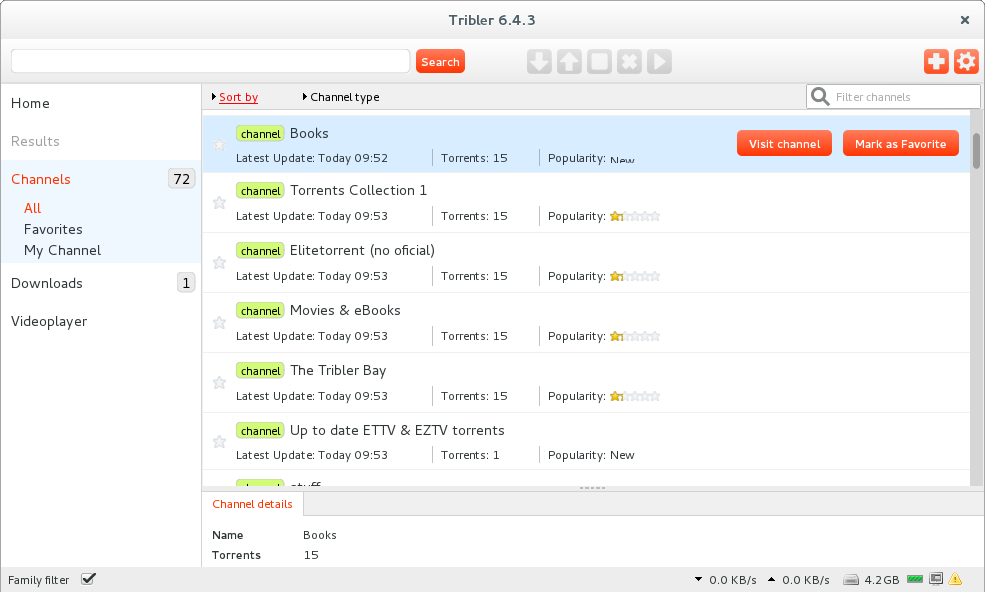
\includegraphics[scale=0.6]{introduction/figs/tribler-screenshot.png}}
	\caption{Screenshot of Tribler v6.4.3.}
	\label{fig:tribler-screenshot}
\end{figure}

\section{Tribler}
In peer-to-peer file sharing a node called a seeder uploads parts
of a file to another node, the downloader.
The seeders and downloaders constantly change
and a node can be both at the same time for different, parallel connections.
A seeder can become a downloader when he wishes to download other files
and downloaders can become seeders,
when they posses a different file someone else wants.
The ratio between the total data downloaded and uploaded is called the seeding ratio~\cite{Cohen-bittorrent}.

Uploading can be seen as an interaction of one node helping another node.
Such interactions come at the cost of consuming bandwidth for both parties.
However, there is only direct benefit for the downloader.
The downloader receives a file he wants.
There is no direct barter between the seeder and downloader.
Because the seeder does not get anything in return for uploading the file.
With a very small chance, can a downloader also be a seeder for the original seeder~\cite{Lai-Incentives}.

Both high availability and high download speeds result in a higher utility for the downloaders.
If everyone contributes, files become more available and are downloaded at higher speed.
This claim is supported by measurements taken in private communities~\cite{meulpolder-privatecommunities}.
In private communities, high seeding ratios are enforced by a tracker.
Trackers are servers where nodes in a peer-to-peer network are introduced to each other,
so that they can upload and download from each other~\cite{cohen-titfortat}.
This tracker can be seen as a central, third party.

But currently freeriding in these networks takes places in high quantities in public networks~\cite{Adar-Freeriding}.
BitTorrent uses a Tit-for-Tat strategy~\cite{cohen-titfortat} to stop freeriding,
but this strategy does not effectively stop abuse~\cite{Pouwelse-tribler}.
The Tit-for-Tat strategy is to only provide help to peers to peers that return this help.

Tribler wants to achieve a high global seeding ratio by making it beneficial to have such a ratio.
Nodes can award each other with higher cooperation if a node has a reputation of being cooperative.
This requires a tamper-proof transaction history capturing previous transactions to base reputation on.
This history has to be available in the network.
Those contributing more receive more help in return,
and malicious nodes cannot abuse the network by tampering with the interaction history.

Within Tribler anonymous connections have been implemented recently using onion routing~\cite{Plak-anonymous,ruigrok-anonymous,tanaskoski-anonymous}.
This feature allows downloaders to become indistinguishable from other users in the network.
Every data packet has to be forwarded
by a number of intermediate hops between the downloader and seeder~\cite{Plak-anonymous,tanaskoski-anonymous}.
The total cost of bandwidth per file is increased,
but also the number of nodes helping a single node downloading a file increases.
The increase in nodes working together increases the necessity of an incentive system to reward collaboration.

Dispersy is middleware for data dissemination in a network.
Dispersy is used heavily within Tribler and is maintained by the Tribler organisation.
Our work is build upon Dispersy.
Dispersy is used to exchange data between two specific nodes~\cite{zeilemaker-dispersy}.
Functionality was added to Dispersy during the thesis.
The additions are described in chapter \ref{chapt:design}.

\section{Document structure}
In chapter 1 we give an overview of Tribler and the organization that develops Tribler.
Chapter 2 gives a description of what the problem is with collaboration in peer-to-peer networks.
Chapter 3 provides an overview of work related to solving the described problem.
The design and implemention of the thesis work is described in chapter 4.
The implementation is tested and the experiments and results are described in chapter 5.
The design has known vulnerabillities and these are explained in chapter 6.
Finally, we discuss the results of our work in chapter 7.
